% Xinzhi: This tikz file is automatically generated by mathcha editor, link: https://www.mathcha.io/editor/Q2WoQCVmFEdfqZCK6qPjLteWJypziy9p08DSxMJpGM







\tikzset{every picture/.style={line width=0.75pt}} %set default line width to 0.75pt        

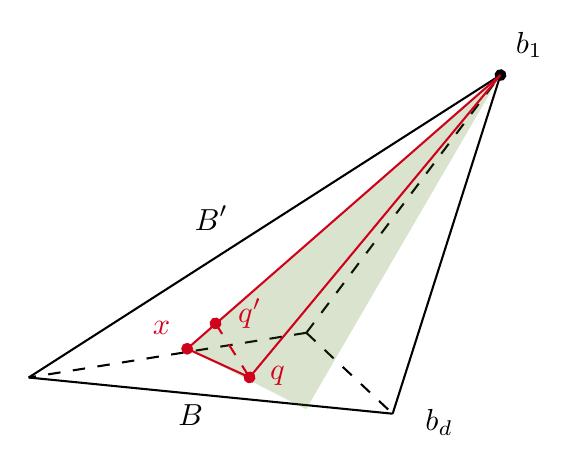
\begin{tikzpicture}[x=0.75pt,y=0.75pt,yscale=-1,xscale=1]
%uncomment if require: \path (0,300); %set diagram left start at 0, and has height of 300

%Straight Lines [id:da3592064404422608] 
\draw    (412.79,90.36) -- (185.5,236.07) ;
\draw [shift={(412.79,90.36)}, rotate = 147.34] [color={rgb, 255:red, 0; green, 0; blue, 0 }  ][fill={rgb, 255:red, 0; green, 0; blue, 0 }  ][line width=0.75]      (0, 0) circle [x radius= 2.34, y radius= 2.34]   ;
%Straight Lines [id:da43460768159824315] 
\draw    (360.84,253.51) -- (185.5,236.07) ;
%Straight Lines [id:da47330666405551947] 
\draw    (360.84,253.51) -- (412.79,90.36) ;
%Straight Lines [id:da33505512651247993] 
\draw  [dash pattern={on 4.5pt off 4.5pt}]  (319.28,214.52) -- (360.84,253.51) ;
%Straight Lines [id:da6293315142262832] 
\draw  [dash pattern={on 4.5pt off 4.5pt}]  (319.28,214.52) -- (185.5,236.07) ;
%Straight Lines [id:da3841197178580813] 
\draw  [dash pattern={on 4.5pt off 4.5pt}]  (319.28,214.52) -- (412.79,90.36) ;
%Shape: Triangle [id:dp6580362388605627] 
\draw  [draw opacity=0][fill={rgb, 255:red, 65; green, 117; blue, 5 }  ,fill opacity=0.2 ][dash pattern={on 0.84pt off 2.51pt}][line width=0.75]  (412.79,90.35) -- (319.15,251.32) -- (261.84,222.22) -- cycle ;
%Straight Lines [id:da35176801472255725] 
\draw [color={rgb, 255:red, 208; green, 2; blue, 27 }  ,draw opacity=1 ] [dash pattern={on 4.5pt off 4.5pt}]  (275.5,210) -- (291.89,236.01) ;
\draw [shift={(291.89,236.01)}, rotate = 57.77] [color={rgb, 255:red, 208; green, 2; blue, 27 }  ,draw opacity=1 ][fill={rgb, 255:red, 208; green, 2; blue, 27 }  ,fill opacity=1 ][line width=0.75]      (0, 0) circle [x radius= 2.34, y radius= 2.34]   ;
\draw [shift={(275.5,210)}, rotate = 57.77] [color={rgb, 255:red, 208; green, 2; blue, 27 }  ,draw opacity=1 ][fill={rgb, 255:red, 208; green, 2; blue, 27 }  ,fill opacity=1 ][line width=0.75]      (0, 0) circle [x radius= 2.34, y radius= 2.34]   ;
%Straight Lines [id:da3023467679043601] 
\draw [color={rgb, 255:red, 208; green, 2; blue, 27 }  ,draw opacity=1 ]   (261.84,222.21) ;
\draw [shift={(261.84,222.21)}, rotate = 0] [color={rgb, 255:red, 208; green, 2; blue, 27 }  ,draw opacity=1 ][fill={rgb, 255:red, 208; green, 2; blue, 27 }  ,fill opacity=1 ][line width=0.75]      (0, 0) circle [x radius= 2.34, y radius= 2.34]   ;
%Straight Lines [id:da6516884798943121] 
\draw [color={rgb, 255:red, 208; green, 2; blue, 27 }  ,draw opacity=1 ]   (412.79,90.36) -- (261.84,222.21) ;
%Straight Lines [id:da6860175398716548] 
\draw [color={rgb, 255:red, 208; green, 2; blue, 27 }  ,draw opacity=1 ]   (291.89,236.01) -- (261.84,222.22) ;
%Straight Lines [id:da24024023553342966] 
\draw [color={rgb, 255:red, 208; green, 2; blue, 27 }  ,draw opacity=1 ]   (291.89,236.01) -- (412.79,90.36) ;

% Text Node
\draw (418.58,68.02) node [anchor=north west][inner sep=0.75pt]  [xscale=1.1,yscale=1.1] [align=left] {$\displaystyle b_{1}$};
% Text Node
\draw (255.93,247.59) node [anchor=north west][inner sep=0.75pt]  [xscale=1.1,yscale=1.1] [align=left] {$\displaystyle B$};
% Text Node
\draw (263.86,151.83) node [anchor=north west][inner sep=0.75pt]  [xscale=1.1,yscale=1.1] [align=left] {$\displaystyle B'$};
% Text Node
\draw (300.11,229.26) node [anchor=north west][inner sep=0.75pt]  [color={rgb, 255:red, 208; green, 2; blue, 27 }  ,opacity=1 ,xscale=1.1,yscale=1.1] [align=left] {$\displaystyle q$};
% Text Node
\draw (284.73,196.33) node [anchor=north west][inner sep=0.75pt]  [color={rgb, 255:red, 208; green, 2; blue, 27 }  ,opacity=1 ,xscale=1.1,yscale=1.1] [align=left] {$\displaystyle \textcolor[rgb]{0.82,0.01,0.11}{q'}$};
% Text Node
\draw (243.62,207.15) node [anchor=north west][inner sep=0.75pt]  [xscale=1.1,yscale=1.1] [align=left] {$\displaystyle \textcolor[rgb]{0.82,0.01,0.11}{x}$};
\draw (375,250) node [anchor=north west][inner sep=0.75pt]  [xscale=1.1,yscale=1.1] [align=left] {$\displaystyle b_{d}$};


\end{tikzpicture}